\documentclass[a4paper, 12pt]{report}
\usepackage{cmap} % поиск в PDF
\usepackage[T2A]{fontenc} % Кодировка
\usepackage[utf8]{inputenc} % Кодировка исходного текста
\usepackage[english,russian]{babel} % Локализация и переносы
\pagestyle{plain} % Для обозначения страниц справа снизу

\usepackage{graphicx}
\graphicspath{ {./images/} }

% Основная часть
\author{Автор: Булат Насыров}
\title{RFT\_CS \\ \footnotesize{\textit{Rocket fuel and trajectory computing system}}}
\date{\today}


\begin{document}
\maketitle

\tableofcontents{}
\clearpage

\chapter{Введение}

\section{Концепция}
\textrm{
    RFT\_CS (Rocket fuel and trajectory computing system) Система расчета ракетного топлива и траектории полета ракеты - это Python-библиотека для разработки математических моделей. RFT\_CS изначально был спроектирован так, чтобы его можно было внедрять постепенно. Другими словами, \textbf{вы можете начать с малого и использовать только ту функциональность RFT\_CS, которая необходима вам в данный момент}. Также в случае, если вам нужно изменить поведение/вычисления функции, есть возможность конфигурации методов под ваши нужды.
}
\section{Цель}
\textrm{
    Основная цель - создать математическую модель процессов, связанных с полётом одно- и многоступенчатых, твердо- и жидкотопливных ракет и для вычисления траектории полёта баллистических ракет.
}
\clearpage

\section{Декомпозиция задачи}
\textrm{
    Начнём с составных частей ракеты, а также внешние факторы, влияющие на полёт. Начнём с состава космической ракеты:
}
\begin{flushright}
    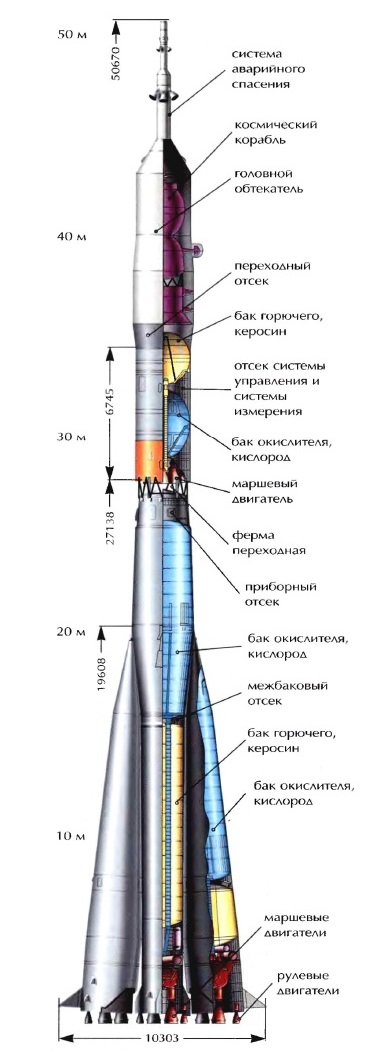
\includegraphics[scale=0.6]{пример_космической_ракеты}
    \label{Рис. 1. Состав космической ракеты}
\end{flushright}
\clearpage
\textrm{Вот состав баллистических ракет: }
\begin{flushright}
    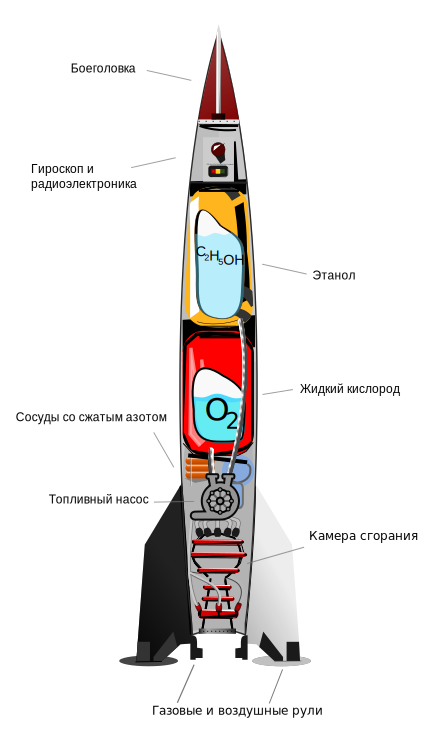
\includegraphics[scale=0.25]{пример_баллистической_ракеты}
    \label{Рис. 2. Состав баллистической ракеты}
\end{flushright}
\end{document}
